%%%%%%%%%%%%%%%%%%%%%%%%%%%%%%%%%%%%

\section{単一割合の推測}

%%%%%%%%%%%%%%%%%%%%%%%%%%%%%%%%%%%%

\begin{frame}

\pq{2人の科学者が、ある薬が高血圧に有効かどうかを調べたいと考えています。1人目の科学者は、高血圧を持つ1000人にその薬を投与し、血圧が下がった人数を記録しようとしています。2人目の科学者は、高血圧を持つ500人に薬を投与し、別の高血圧を持つ500人には投与しないで、両グループで血圧が下がった人数を比較しようとしています。この薬を試験するためにより良い方法はどちらですか？}

\begin{enumerate}[(a)]
\item 1000人全員に薬を投与する
\solnMult{500人に投与し、500人には投与しない}
\end{enumerate}

\end{frame}

%%%%%%%%%%%%%%%%%%%%%%%%%%%%%%%%%%%%

\begin{frame}
\frametitle{GSSの結果}

GSSは同じ質問を行っており、以下は2010年の調査の回答の分布です：\\

\begin{center}
\begin{tabular}{l c}
1000人全員に薬を投与する		& 99 \\
500人に投与し、500人には投与しない	& 571 \\
\hline
合計					& 670
\end{tabular}
\end{center}

\end{frame}

%%%%%%%%%%%%%%%%%%%%%%%%%%%%%%%%%%%

\begin{frame}
\frametitle{母数（パラメータ）と点推定値}

\dq{実験計画について正しい直感を持つ、つまり「500人に投与し、500人には投与しない」と答えるアメリカ人全体の割合を推定したいと思います。関心のある母数（パラメータ）と点推定値は何ですか？}

\begin{itemize}

\item \hl{関心のある母数（パラメータ）：}\orange{全}アメリカ人のうち、実験計画について正しい直感を持つ人の割合。
\[ \mathhl{p}~\scriptsize{(\text{母集団の割合})} \]

\item \hl{点推定値：}\orange{標本抽出された}アメリカ人のうち、実験計画について正しい直感を持つ人の割合。
\[ \mathhl{\hat{p}}~\scriptsize{(\text{標本の割合})} \]

\end{itemize}

\end{frame}

%%%%%%%%%%%%%%%%%%%%%%%%%%%%%%%%%%%

\begin{frame}
\frametitle{割合の推測}

\dq{実験計画について正しい直感を持つ、つまり「500人に投与し、500人には投与しない」と答えるアメリカ人全体の割合は何パーセントですか？}

\begin{itemize}

\item この研究上の問いは信頼区間を使って答えることができます。信頼区間は常に次の形をとります：

\[ \textcolor{orange}{点推定値 \pm 誤差の範囲} \]

\item また、\textcolor{orange}{$誤差の範囲 = 臨界値 \times 点推定値の標準誤差$}であることも知っています。

\end{itemize}

\formula{標本割合の標準誤差}
{
\[ SE_{\hat{p}} =  \sqrt{\frac{p~(1-p)}{n}}  \]
}


\end{frame}

%%%%%%%%%%%%%%%%%%%%%%%%%%%%%%%%%%%

\subsection{標本割合がほぼ正規分布に従う場合の確認}

%%%%%%%%%%%%%%%%%%%%%%%%%%%%%%%%%%%%

\begin{frame}
\frametitle{標本割合もほぼ正規分布に従う}

\formula{割合の中心極限定理}
{
標本割合は、母集団の割合$p$を平均とし、標準誤差$\sqrt{\frac{p~(1-p)}{n}}$を持つ正規分布にほぼ従います。
\[ \hat{p} \sim N \pr{ mean = p, SE = \sqrt{\frac{p~(1-p)}{n}} } \]
}

もちろん、これはある条件のもとでのみ成り立ちます…

\dq{何か予想できますか？}

\soln{独立な観測値、少なくとも10の成功と10の失敗}

\Note{$p$が未知の場合（ほとんどのケース）、標準誤差の計算に$\hat{p}$を使用します。}

\end{frame}

%%%%%%%%%%%%%%%%%%%%%%%%%%%%%%%%%%%

\subsection{割合の信頼区間}

%%%%%%%%%%%%%%%%%%%%%%%%%%%%%%%%%%%%

\begin{frame}
\frametitle{実験計画の話に戻ろう…}

\dq{GSSによると、670人中571人（85\%）のアメリカ人が実験計画に関する質問に正しく回答しました。実験計画について正しい直感を持つアメリカ人全体の割合を、95\%信頼区間を用いて推定してください。}

与えられた値：$n = 670, \hat{p} = 0.85$。まず条件を確認します。

\begin{enumerate}[1.]
\item \hl{独立性：}標本は無作為に抽出されており、670 $<$ 全アメリカ人の10\%であるため、ある回答者の回答が別の回答者の回答と独立していると仮定できます。
\item \hl{成功・失敗条件：}571人が正しく回答（成功）し、99人が誤って回答（失敗）しており、両方とも10以上です。
\end{enumerate}

\end{frame}

%%%%%%%%%%%%%%%%%%%%%%%%%%%%%%%%%%%

\begin{frame}

\pq{$n = 670, \hat{p} = 0.85$が与えられており、標本割合の標準誤差は$SE = \sqrt{\frac{p(1-p)}{n}}$であることを学びました。95\%信頼区間の正しい計算式はどれですか？}

\begin{enumerate}[(a)]
\solnMult{$0.85 \pm 1.96 \times \sqrt{\frac{0.85 \times 0.15}{670}}$} \only<2->{\orange{$\rightarrow (0.82, 0.88)$}}
\item $0.85 \pm 1.65 \times \sqrt{\frac{0.85 \times 0.15}{670}}$
\item $0.85 \pm 1.96 \times \frac{0.85 \times 0.15}{\sqrt{670}}$
\item $571 \pm 1.96 \times \sqrt{\frac{571 \times 99}{670}}$
\end{enumerate}

\end{frame}

%%%%%%%%%%%%%%%%%%%%%%%%%%%%%%%%%%

%%%%%%%%%%%%%%%%%%%%%%%%%%%%%%%%%%%

\subsection{割合を推定する際の標本サイズの選択}

%%%%%%%%%%%%%%%%%%%%%%%%%%%%%%%%%%%

\begin{frame}
\frametitle{標本サイズの選択}

\dq{95\%信頼区間の誤差の範囲を1\%に抑えるためには、何人を標本抽出する必要がありますか？}
\[ ME = z^\star \times SE\]
\begin{eqnarray*}
0.01 &\ge& 1.96 \times \sqrt{\frac{0.85 \times 0.15}{n}} \orange{$\rightarrow$ \text{前の研究の$\hat{p}$を使用}} \\
0.01^2 &\ge& 1.96^2 \times \frac{0.85 \times 0.15}{n} \\
n &\ge& \frac{1.96^2 \times 0.85 \times 0.15}{0.01^2} \\
n &\ge& 4898.04 \orange{~$\rightarrow$ nは少なくとも4,899必要}
\end{eqnarray*}

\end{frame}

%%%%%%%%%%%%%%%%%%%%%%%%%%%%%%%%%%%

\begin{frame}
\frametitle{過去の研究がない場合は？}

… $\hat{p} = 0.5$を使用します

\vspace{1cm}

\dq{なぜですか？}

\begin{itemize}
\item 何もわからない場合、50-50が最も合理的な推測です
\item $\hat{p} = 0.5$は最も保守的な推定値を与えます — 最大の標本サイズが必要
\end{itemize}

\end{frame}

%%%%%%%%%%%%%%%%%%%%%%%%%%%%%%%%%%%%

\subsection{割合の仮説検定}

%%%%%%%%%%%%%%%%%%%%%%%%%%%%%%%%%%%%%

\begin{frame}
\frametitle{割合のCIとHT}

\begin{itemize}

\item 成功・失敗条件：
\begin{itemize}
\item CI：少なくとも10の\orange{観測された}成功と失敗
\item HT：帰無値を使って計算した、少なくとも10の\orange{期待される}成功と失敗
\end{itemize}

\item 標準誤差：
\begin{itemize}
\item CI：観測された標本割合を使って計算：$SE = \sqrt{\frac{\hat{p}(1-\hat{p})}{n}}$
\item HT：帰無値を使って計算：$SE = \sqrt{\frac{p_0(1-p_0)}{n}}$
\end{itemize}

\end{itemize}

\end{frame}

%%%%%%%%%%%%%%%%%%%%%%%%%%%%%%%%%%%

\begin{frame}
\frametitle{}

\dq{GSSによると、670人中571人（85\%）のアメリカ人が実験計画に関する質問に正しく回答しました。このデータは、80\%以上のアメリカ人が実験計画について正しい直感を持つという説得力のある証拠を提供しますか？}

\[ H_0: p = 0.80 \qquad H_A: p > 0.80 \]

\twocol{0.6}{0.4}
{
\begin{eqnarray*}
SE &=& \sqrt{\frac{0.80 \times 0.20}{670}} = 0.0154 \\
Z &=& \frac{0.85 - 0.80}{0.0154} = 3.25 \\
p\text{値} &=& 1 - 0.9994 = 0.0006 \\
\end{eqnarray*}
}
{
\begin{center}
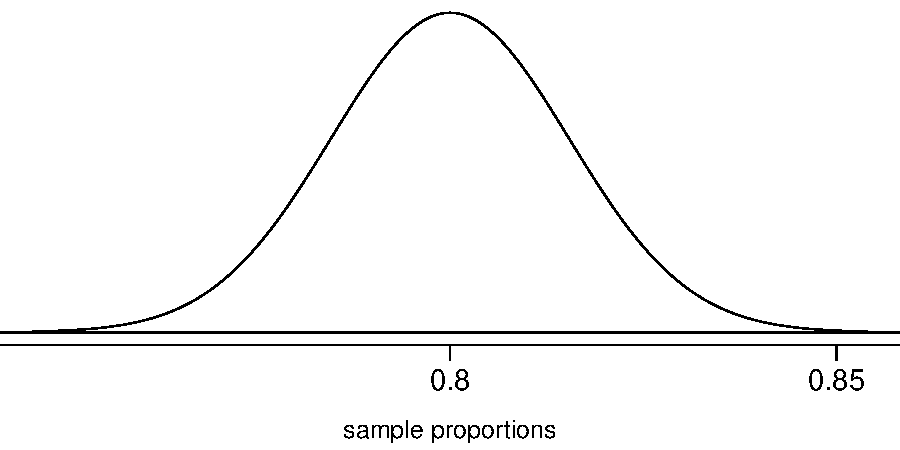
\includegraphics[width=\textwidth]{6-1_single_prop/figures/expdesgn_norm}
\end{center}
}
p値が低いため、$H_0$を棄却します。このデータは、80\%以上のアメリカ人が実験計画について正しい直感を持つという説得力のある証拠を提供します。

\end{frame}

%%%%%%%%%%%%%%%%%%%%%%%%%%%%%%%%%%%

\subsection{まとめ}

%%%%%%%%%%%%%%%%%%%%%%%%%%%%%%%%%%%

\begin{frame}
\frametitle{}

\pq{2006年のギャラップ調査に回答した1,001人のアメリカ人のうち、11\%が宗教的な理由からハロウィンのお祝いに反対していると回答しました。95\%信頼水準で、この調査の誤差の範囲は$\pm 3\%$です。この研究結果に関するニュース記事には「10\%以上のアメリカ人が宗教的な理由からハロウィンのお祝いに反対している」と書かれています。95\%信頼水準で、このニュース記事の主張は正当化されますか？}

\begin{enumerate}[(a)]
\item はい
\solnMult{いいえ}
\item 判断できない
\end{enumerate}

\end{frame}

%%%%%%%%%%%%%%%%%%%%%%%%%%%%%%%%%%

\begin{frame}
\frametitle{まとめ - 1つの割合の推測}

\begin{itemize}

\item 母集団のパラメータ：$p$、点推定値：$\hat{p}$

\item 条件：
\begin{itemize}
\item 独立性 \\
- 無作為標本かつ10\%条件
\item 少なくとも10の成功と失敗\\ - 満たさない場合 $\rightarrow$ 無作為化
\end{itemize}

\item 標準誤差：$SE = \sqrt{ \frac{p(1-p)}{n} }$
\begin{itemize}
\item CIの場合：$\hat{p}$を使用
\item HTの場合：$p_0$を使用
\end{itemize}

\end{itemize}

\end{frame}
